\documentclass{beamer}

\usepackage[english]{babel}
\usepackage[utf8]{inputenc}
\usepackage{caption}

\usetheme{Madrid}
\usecolortheme{default}

\setbeamertemplate{bibliography entry title}{}
\setbeamertemplate{bibliography entry location}{}
\setbeamertemplate{bibliography entry note}{}

\title[Project 2221]{Designing Scientific Applications on GPUs}
\subtitle{CUDA implementation of the LibRSB library}
\author[Filippo Barbari]{Filippo Barbari}
\institute[LUX]{University of Luxembourg}
\date[Summer School 2022]{PRACE's Summer School of HPC 2022}

\AtBeginSection[]
{
	\begin{frame}
		\frametitle{Table of Contents}
		\tableofcontents[currentsection]
	\end{frame}
}

\begin{document}
	
	\frame{\titlepage}
	
	\begin{frame}{Table of Contents}
		\tableofcontents
	\end{frame}
	
	\section{LibRSB}
	\begin{frame}{LibRSB}
		LibRSB implements some common sparse matrices operations in a cache-efficient and parallel way using the Recursive Sparse Blocks format storage format.
		\begin{itemize}
			\item \textbf{SpVV}: sparse vector to dense vector multiplication
			\item \textbf{SpMV}: sparse matrix to dense vector multiplication
			\item \textbf{SpMM}: sparse matrix to matrix multiplication
			\item \textbf{SpSM}: solving a sparse matrix to matrix linear system
			\item \textbf{SpSV}: solving a sparse matrix to dense vector linear system
		\end{itemize}
	\end{frame}
	
	\begin{frame}{What is Recursive Sparse Blocks?}
		As explained in \cite{martone2010utilizing} (paragraph 2.1, Matrix Partitioning), RSB is a hybrid format which combines three different storage formats together at different levels:
		\begin{enumerate}
			\item \textit{at the high level}, \textbf{Z Morton sorting} of blocks
			\item \textit{at the intermediate level}, blocks are recursively subdivided in a \textbf{Quad-tre} structure
			\item \textit{at the leaf level}, each submatrix/block is stored with the standard \textbf{COO/CSR/CSC} formats
		\end{enumerate}
	\end{frame}
	
	\subsection{Z Morton sorting}
	\begin{frame}{Z Morton sorting}
		\begin{minipage}{.48\textwidth}
			It’s a special kind of mathematical \textbf{space filling curve} (like Hilbert’s spiral) which preserves spatial locality of the data points.\\
			
			\bigskip
			Spatial locality is important because it improves the hit/miss ratio of the cache.
		\end{minipage}
		\hfill
		\begin{minipage}{.48\textwidth}
			\begin{figure}
				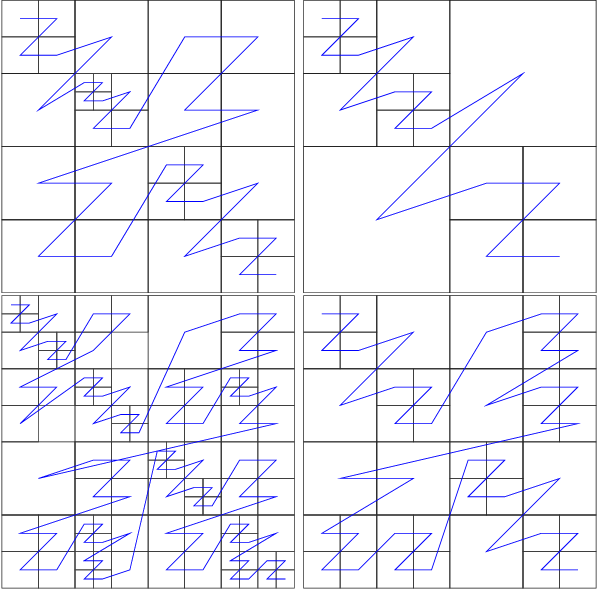
\includegraphics[scale=0.27]{zmorton}
				\caption*{{\tiny Z Morton sorting of two different matrices (up and down) with two different granularities (left and right).}}
			\end{figure}
		\end{minipage}
	\end{frame}
	
	\subsection{Quad-tree}
	\begin{frame}{Quad-tree}
		\begin{minipage}{.48\textwidth}
			{\small A quad-tree is a quaternary tree often used to subdivide continuous space in order to optimize a “look around” query. The RSB format uses it to find the non-zero blocks/submatrices inside the discretized space of matrix coordinates.\\
			
			\bigskip
			The original author, Michele Martone, uses an heuristic to determine whether to subdivide a given block or not based on the number of non-zero elements inside it and the L3 cache size of the machine the algorithm is being executed on.}
		\end{minipage}
		\hfill
		\begin{minipage}{.48\textwidth}
			\begin{figure}
				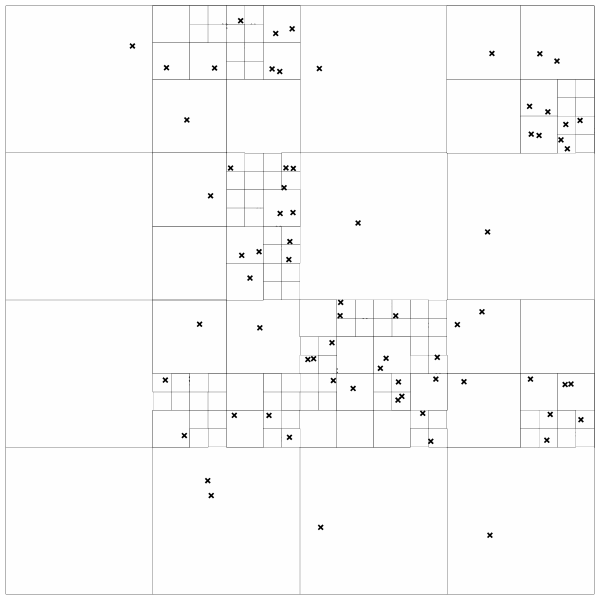
\includegraphics[scale=0.27]{quad-tree}
				\caption*{{\tiny An example of Quad-tree for 2D points in a continuous space.}}
			\end{figure}
		\end{minipage}
	\end{frame}
	
	\subsection{COO/CSR/CSC formats}
	\begin{frame}{COO format}
		These are the most commonly used formats to memorize sparse matrices/vectors.
		\begin{itemize}
			\item \textbf{COOrdinate list} represents a matrix as an array of triplets each having:
			\begin{itemize}
				\item[-] the row index of the non-zero element
				\item[-] the column index of the non-zero element
				\item[-] the value
			\end{itemize}
		\end{itemize}
		For example, the matrix on the left is stored as shown on the right.\\
		
		\bigskip
		\begin{minipage}{.48\textwidth}
			\begin{center}
				$\begin{bmatrix}
					0 & 0 & 3 & 0 & 0 \\
					0 & 0 & 0 & 7 & 0 \\
					0 & 2 & 0 & 0 & 0 \\
					0 & 6 & 0 & 0 & 1 \\
					0 & 0 & 5 & 0 & 0 \\
				\end{bmatrix}$
			\end{center}
		\end{minipage}
		\hfill
		\begin{minipage}{.48\textwidth}
			\begin{center}
				\def\arraystretch{2}
				\begin{tabular}{|c|c|c|c|c|c|c|}
					\hline
					row idx & 0 & 1 & 2 & 3 & 3 & 4 \\
					\hline
					col idx & 2 & 3 & 1 & 1 & 4 & 2 \\
					\hline
					value & 3 & 7 & 2 & 6 & 1 & 5 \\
					\hline
				\end{tabular}
			\end{center}
		\end{minipage}
	\end{frame}
	
	\begin{frame}{CSR format}
		\begin{itemize}
			\item \textbf{Compressed Sparse Rows} works the same way of COO but it compresses contiguous row indices by memorizing the indices in the col\_idx array which contain the elements in each row.
			
			\bigskip
			CSR uses less memory than COO only if the non-zero elements are denser on the rows than the columns.
		\end{itemize}
		For example, the previous matrix requires one less index.\\
		
		\bigskip
		\begin{minipage}{.48\textwidth}
			\begin{center}
				$\begin{bmatrix}
					0 & 0 & 3 & 0 & 0 \\
					0 & 0 & 0 & 7 & 0 \\
					0 & 2 & 0 & 0 & 0 \\
					0 & 6 & 0 & 0 & 1 \\
					0 & 0 & 5 & 0 & 0 \\
				\end{bmatrix}$
			\end{center}
		\end{minipage}
		\hfill
		\begin{minipage}{.48\textwidth}
			\begin{center}
				\def\arraystretch{2}
				\begin{tabular}{|c|c|c|c|c|c|c}
					\cline{1-6}
					row idx & 0 & 1 & 2 & 3 & 4 &                        \\ \hline
					col idx & 2 & 3 & 1 & 1 & 4 & \multicolumn{1}{c|}{2} \\ \hline
					value   & 3 & 7 & 2 & 6 & 1 & \multicolumn{1}{c|}{5} \\ \hline
				\end{tabular}
			\end{center}
		\end{minipage}
	\end{frame}
	
	\begin{frame}{CSC format}
		\begin{itemize}
			\item \textbf{Compressed Sparse Columns} works the same way of CSR but compresses the column indices instead.
			
			\bigskip
			Usually, CSC is used in some rare cases where the matrix is stored in column-major ordering.
		\end{itemize}
		For example, the previous matrix requires two less column indices.\\
		
		\bigskip
		\begin{minipage}{.48\textwidth}
			\begin{center}
				$\begin{bmatrix}
					0 & 0 & 3 & 0 & 0 \\
					0 & 0 & 0 & 7 & 0 \\
					0 & 2 & 0 & 0 & 0 \\
					0 & 6 & 0 & 0 & 1 \\
					0 & 0 & 5 & 0 & 0 \\
				\end{bmatrix}$
			\end{center}
		\end{minipage}
		\hfill
		\begin{minipage}{.48\textwidth}
			\begin{center}
				\def\arraystretch{2}
				\begin{tabular}{|c|c|c|c|c|cc}
					\cline{1-5}
					col idx & 0 & 2 & 3 & 4 &                        &                        \\ \hline
					row idx & 2 & 3 & 0 & 4 & \multicolumn{1}{c|}{1} & \multicolumn{1}{c|}{3} \\ \hline
					value   & 2 & 6 & 3 & 5 & \multicolumn{1}{c|}{7} & \multicolumn{1}{c|}{1} \\ \hline
				\end{tabular}
			\end{center}
		\end{minipage}
	\end{frame}
	
	\section{Analysis}
	\begin{frame}{Analysis}
		TODO
	\end{frame}
	
	\section{Design}
	\begin{frame}{Design}
		TODO
	\end{frame}
	
	\section{Implementation}
	\begin{frame}{Implementation}
		TODO
	\end{frame}
	
	\section{Performance Evaluation}
	\begin{frame}{Performance Evaluation}
		TODO
	\end{frame}
	
	\section{Conclusions}
	\begin{frame}{Conclusions}
		TODO
	\end{frame}
	
	\section{Future work}
	\begin{frame}{Future work}
		TODO
	\end{frame}
	
	\begin{frame}[allowframebreaks]
		\frametitle{References}
		\bibliographystyle{amsalpha}
		\bibliography{references.bib}
	\end{frame}
	
\end{document}